\section{Pianificazione}

Al fine della pianificazione si è deciso di suddividere il progetto in cinque macro-fasi distinte:
\begin{itemize}
\item \textbf{\AR:} fase di analisi iniziale;
\item \textbf{\AD:} fase di analisi successiva all'accettazione della proposta;
\item \textbf{\PA}
\item \textbf{\PD e \Cod}
\item \textbf{\VV}
\end{itemize}
Ogni macro-fase è stata poi suddivisa in sotto-attività, ad ognuna delle quali sono assegnate una o più risorse. Le attività sono rappresentate attraverso diagrammi di \glossario{Gantt}. Nei diagrammi sono presenti anche le \glossario{milestone}, a rappresentare la conclusione dell'attività coincidente con la consegna dei documenti. \\
Per il glossario non è stata prevista alcuna ripartizione delle ore tra i componenti del gruppo per la redazione in quanto viene redatto contemporaneamente alla stesura degli altri documenti ogni qualvolta un termine necessiti di una spiegazione.

\subsection{\AR}
\textbf{Periodo:} da 10-12-2016 a 11-01-2017 \\
Tale fase inizia in corrispondenza della data di scadenza per la formazione dei gruppi e termina con la data di consegna dei documenti per la \RR. Nella fase di \AR{} i documenti di maggior impatto sono: \textit{Norme di progetto}, \textit{Studio di fattibilità}, \textit{Analisi dei requisiti}, \textit{Piano di qualifica}, \textit{Piano di progetto}, \textit{Glossario} e \textit{Lettera di presentazione}.
Nella fase di Analisi i ruoli maggiormente coinvolti sono \Analista{}, \Responsabile{}, \Amministratore{} e \Verificatore{}.

\subsubsection{Gantt attività}
\begin{figure}[H]
\centering
\scalebox{0.3}{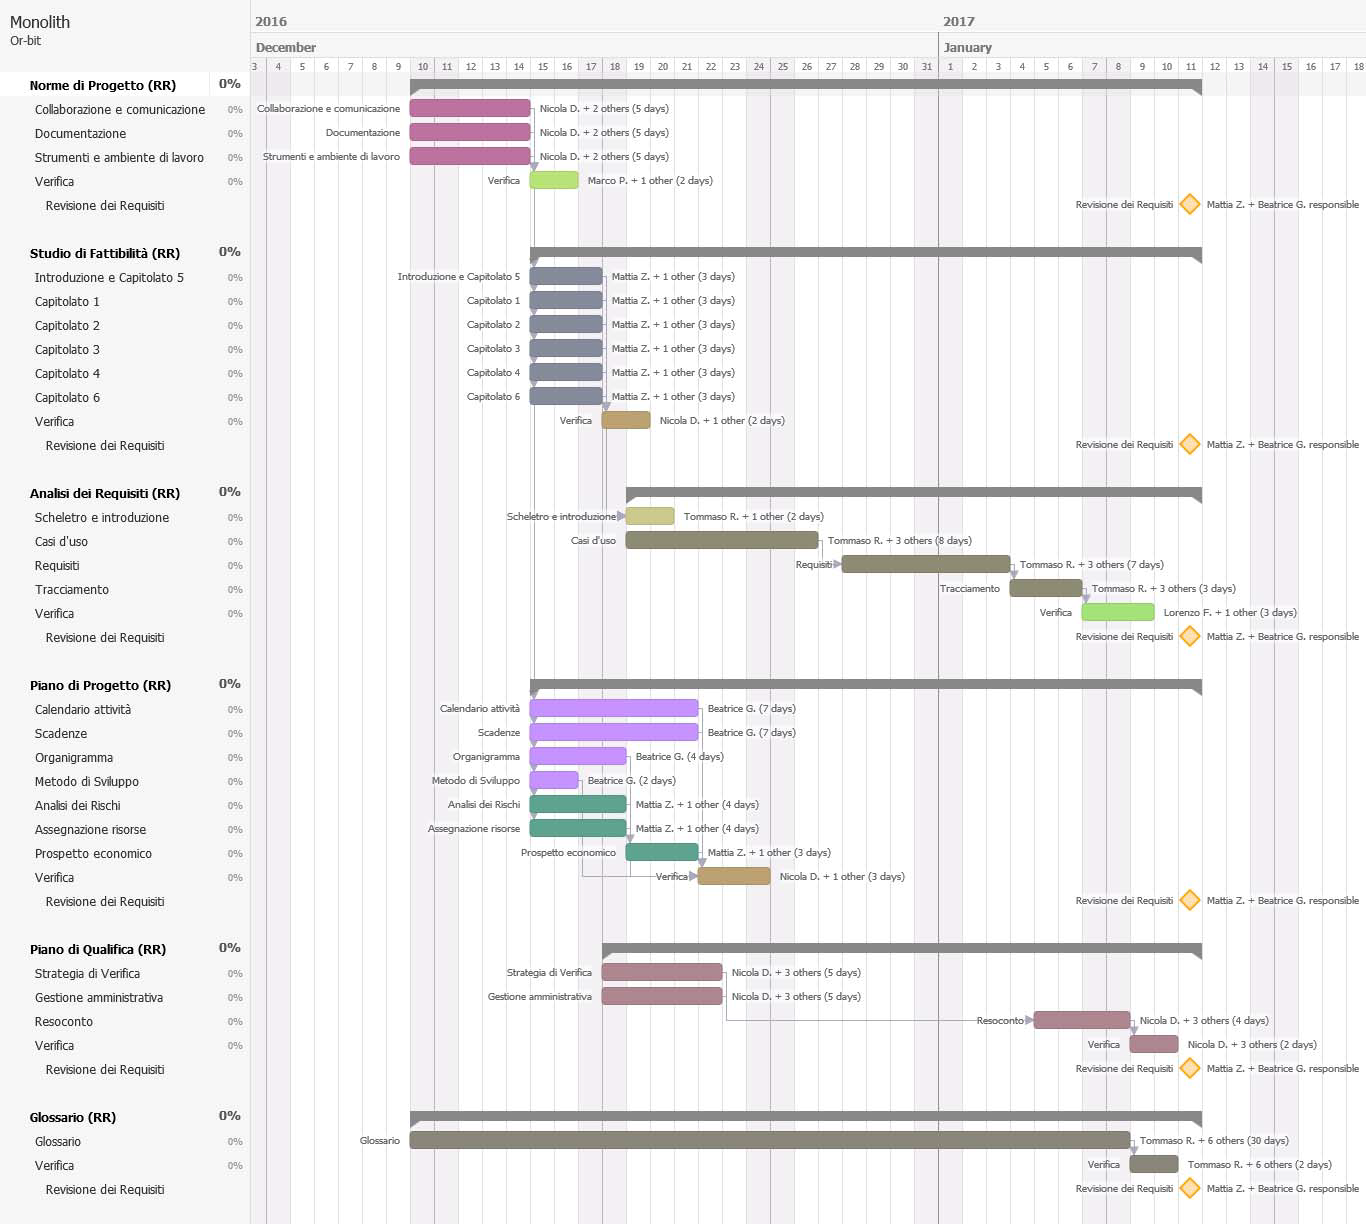
\includegraphics{gantt/Gantt_RR.png}}
\caption{Diagramma di Gantt, fase di \AR{}}
\end{figure}

\subsubsection{Ripartizione ore}
\bgroup
\begin{longtable}{|l|l|l|c|}
  \endfirsthead
  \hline
  \textbf{Identificativo} &
  \textbf{Nome Attività} &
  \textbf{Ruolo} &
  \textbf{Ore}\\
  \endhead
  \hline
  \textbf{AN1} & \textbf{Norme di Progetto} &  &  \\
  \hline
  	{AN1.1} & {Collaborazione e comunicazione} & Amministratore  & 3\\
  	\hline
  	{AN1.2} & {Documentazione} & Amministratore & 6\\
  	\hline
  	{AN1.3} & {Strumenti e ambiente di lavoro} & Amministratore &  1\\
  	\hline
  	{AN1.4} & {Verifica} & Verificatore & 3 \\
  \hline
  \textbf{AN2} & \textbf{Piano di Progetto}  & & \\
    \hline
    	{AN2.1} & {Calendario attività} & Responsabile &  5\\
    	\hline
    	{AN2.2} & {Scadenze} & Responsabile & 3 \\
    	\hline
    	{AN2.3} & {Organigramma} & Responsabile & 2 \\
    	\hline
    	{AN2.4} & {Metodo di sviluppo} & Responsabile &   3\\
    	\hline
    	{AN2.5} & {Analisi dei rischi} & Responsabile  &  5\\
    	\hline
    	{AN2.6} & {Assegnazione risorse} & Responsabile  &  5\\
    	\hline
    	{AN2.7} & {Prospetto Economico} & Responsabile  &  4\\
    	\hline
    	{AN2.8} & {Verifica} & Verificatore & 3 \\
    \hline
    \textbf{AN3} & \textbf{Studio di Fattibilità}  & &  \\
      \hline
      	{AN3.1} & {Introduzione e Capitolato 5} & Analista  & 3 \\
      	\hline
      	{AN3.2} & {Capitolato 1} & Analista & 3\\
      	\hline
      	{AN3.3} & {Capitolato 2} & Analista  & 3 \\
      	\hline
      	{AN3.4} & {Capitolato 3} & Analista  & 3 \\
      	\hline
      	{AN3.5} & {Capitolato 4} & Analista  & 3 \\
      	\hline
      	{AN3.6} & {Capitolato 5} & Analista  & 3 \\
      	\hline
      	{AN3.7} & {Capitolato 6} & Analista  & 3 \\
      	\hline
      	{AN3.8} & {Verifica} & Verificatore  & 2 \\
      \hline
      \textbf{AN4} & \textbf{Analisi dei Requisiti} & &  \\
         \hline
         {AN4.1} & {Scheletro e introduzione} & Analista  &  9\\
         \hline
         {AN4.2} & {Casi d'uso} & Analista  &  9\\
         \hline
         {AN4.3} & {Requisiti} & Analista  &  15\\
         \hline
         {AN4.4} & {Tracciamento} & Analista  &  6\\
         \hline
         {AN4.5} & {Verifica} & Verificatore  & 6\\
     \hline
     \textbf{AN5} & \textbf{Piano di Qualifica} & &  \\
         \hline
         {AN5.1} & {Strategia e Verifica} & Analista &  6 \\
         & & Responsabile & 6\\
         & & Verificatore & 6\\
         \hline
         {AN5.2} & {Gestione amministrativa} & Amministratore & 6\\
         & & Analista & 6\\
         & & Responsabile & 6\\
         & & Verificatore & 6\\
         \hline
         {AN5.3} & {Resoconto} & Verificatore &  3\\
         \hline
         {AN5.4} & {Verifica} & Verificatore &  3 \\
     \hline
     \textbf{AN6} & \textbf{Glossario} & &  \\
         \hline
         {AN6.1} & {Verifica} & Verificatore &  3 \\
         \hline
     \\
     \caption{Ripartizione ore fase di \AR}
\end{longtable}
\egroup
  
\subsection{\AD}
\textbf{Periodo:} da 25-01-2017 a 28-01-2017 \\
Tale fase inizia in corrispondenza della revisione dei requisiti. La fase di \AD{} riguarda un incremento e correzione dei documenti stilati durante la fase di \AR{}: \textit{Norme di progetto}, \textit{Analisi dei requisiti}, \textit{Piano di qualifica}, \textit{Piano di progetto} e \textit{Glossario}.
Nella fase di \AD{} i ruoli maggiormente coinvolti sono \Analista{}, \Responsabile{}, \Amministratore{} e \Verificatore{}.

\subsubsection{Gantt attività}
\begin{figure}[H]
	\centering
	\scalebox{0.3}{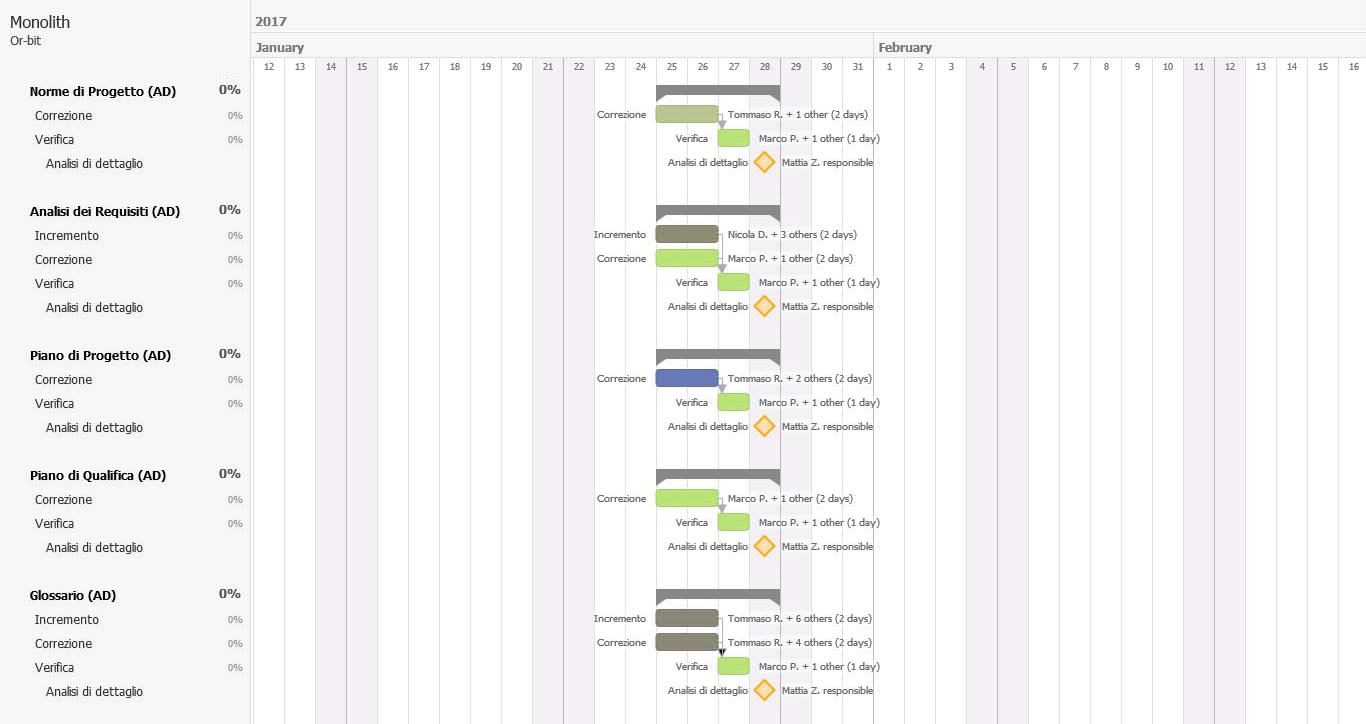
\includegraphics{gantt/Gantt_AD.png}}
	\caption{Diagramma di Gantt, fase di \AD{}}
\end{figure}

\subsubsection{Ripartizione ore}
\bgroup
\begin{longtable}{|l|l|l|c|}
	\endfirsthead
	\hline
	\textbf{Identificativo} &
	\textbf{Nome Attività} &
	\textbf{Ruolo} &
	\textbf{Ore}\\
	\endhead
	\hline
	\textbf{AD1} & \textbf{Norme di Progetto} &  &  \\
		\hline
		{AD1.1} & {Correzione} & Amministratore  & 1\\
		\hline
		{AD1.4} & {Verifica} & Verificatore & 1 \\
		\hline
	\textbf{AD2} & \textbf{Piano di Progetto}  & & \\
	\hline
		{AD2.1} & {Correzione} & Responsabile &  1\\
		\hline
		{AD2.2} & {Verifica} & Verificatore & 0.5 \\
		\hline
	\textbf{AD3} & \textbf{Analisi dei Requisiti} & &  \\
		\hline
		{AD3.1} & {Correzione} & Analista  &  5\\
		\hline
		{AD3.2} & {Incremento} & Analista  &  5\\
		\hline
		{AD3.3} & {Verfica} & Verificatore  &  1.5\\
		\hline
	\textbf{AD4} & \textbf{Piano di Qualifica} & &  \\
	\hline
		{AD4.1} & {Correzione} & Analista &  5 \\
		\hline
		{AD4.2} & {Verifica} & Verificatore &  0.5 \\
		\hline
	\textbf{AD5} & \textbf{Glossario} & &  \\
	\hline
		{AD5.1} & {Verifica} & Verificatore &  0.5 \\
	\hline
	\\
	\caption{Ripartizione ore fase di \AD}
\end{longtable}
\egroup

\subsection{\PA}
\textbf{Periodo:} da 29-01-2017 a 06-03-2017 \\
Tale fase inizia dopo la fase di \AD{}. La fase di \textbf{Progettazione architetturale} riguarda lo sviluppo dell'architettura del sistema da realizzare. I documenti che vengono incrementati in questa fase sono: \textit{Specifica Tecnica}, accompagnata da: \textit{Norme di progetto}, \textit{Piano di qualifica} e \textit{Glossario}.
Nella fase di \PA{} i ruoli maggiormente coinvolti sono \Progettista{}, \Responsabile{}, \Amministratore{}, \Analista{} e \Verificatore{}.
\subsubsection{Gantt attività}
\begin{figure}[H]
	\centering
	\scalebox{0.3}{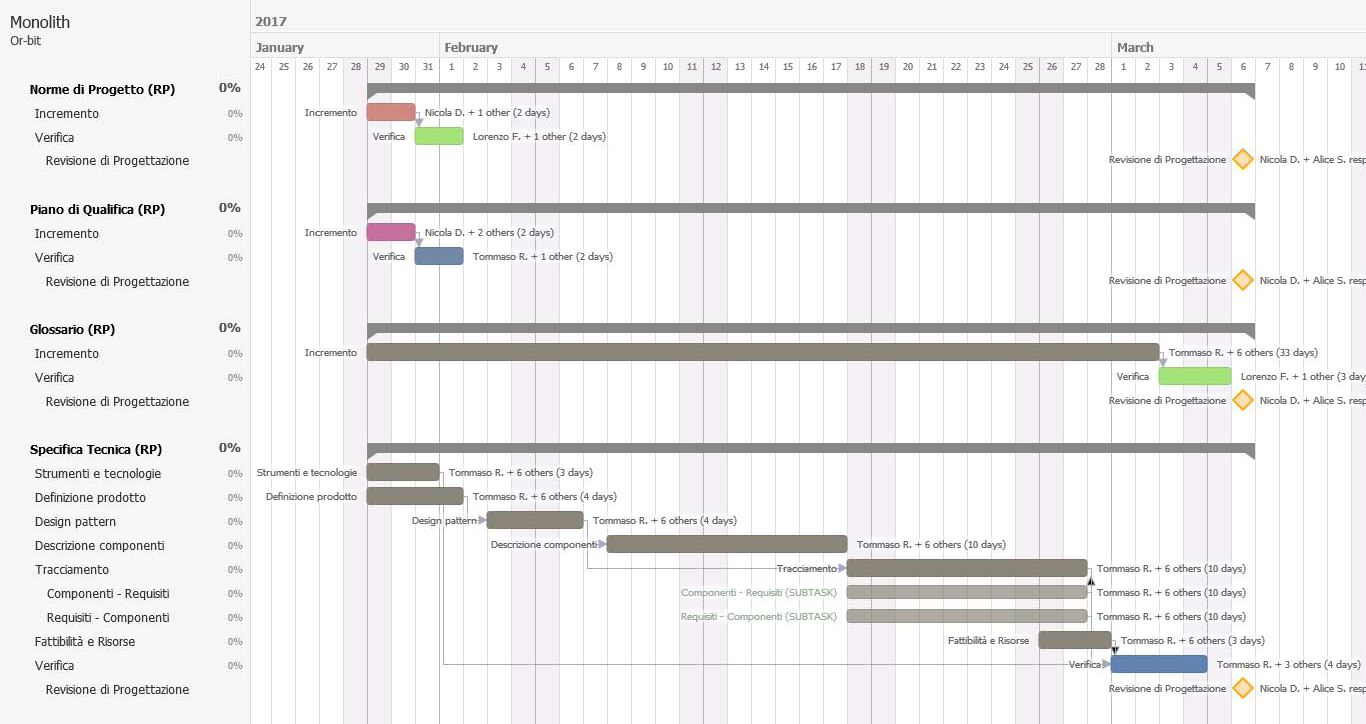
\includegraphics{gantt/Gantt_RP.png}}
	\caption{Diagramma di Gantt, fase di \PA{}}
\end{figure}

\subsubsection{Ripartizione ore}
\bgroup
\begin{longtable}{|l|l|l|c|}
	\endfirsthead
	\hline
	\textbf{Identificativo} &
	\textbf{Nome Attività} &
	\textbf{Ruolo} &
	\textbf{Ore}\\
	\endhead
	\hline
	\textbf{RP1} & \textbf{Norme di Progetto} &  &  \\
	\hline
	{RP1.1} & {Incremento} & Amministratore  & 3\\
	\hline
	{RP1.2} & {Verifica} & Verificatore & 5 \\
	\hline
	\textbf{RP2} & \textbf{Piano di Qualifica}  & & \\
	\hline
	{RP2.1} & {Incremento} & Responsabile &  3\\
	\hline
	{RP2.2} & {Verifica} & Verificatore & 5 \\
	\hline
	\textbf{RP3} & \textbf{Specifica tecnica} & &  \\
	\hline
	{RP3.1} & {Strumenti e tecnologie} & Amministratore  &  2\\
	& & Progettista & 7 \\
	\hline
	{RP3.2} & {Definizione di prodotto} & Progettista  &  5\\
	\hline
	{RP3.3} & {Design pattern} & Progettista  &  25\\
	\hline
	{RP3.4} & {Descrizione componenti} & Progettista  &  25\\
	\hline
	{RP3.5} & {Tracciamento} & Progettista  &  20\\
	& & Analista & 15 \\
	\hline
	{RP3.6} & {Fattibilità e Risorse} & Responsabile  &  2\\
	& & Progettista & 5 \\
	\hline
	{RP3.7} & {Verifica} & Verificatore  &  25\\
	\hline
	\textbf{RP4} & \textbf{Glossario} & &  \\
	\hline
	{RP4.1} & {Verifica} & Verificatore &  4 \\
	\hline
	\\
	\caption{Ripartizione ore fase di \PA}
\end{longtable}
\egroup

\subsection{\PD e \Cod}
\textbf{Periodo:} da 14-03-2017 a 11-04-2017 \\
 La fase di \PD{} e \Cod{} riguarda un incremento e correzione dei documenti finora stilati e lo sviluppo del sistema da realizzare.
Nella fase di \PD{} e \Cod{} i ruoli maggiormente coinvolti sono \Programmatore{}, \Progettista{}, \Analista{}, \Responsabile{}, \Amministratore{} e \Verificatore{}.
\subsubsection{Gantt attività}
\begin{figure}[H]
	\centering
	\scalebox{0.3}{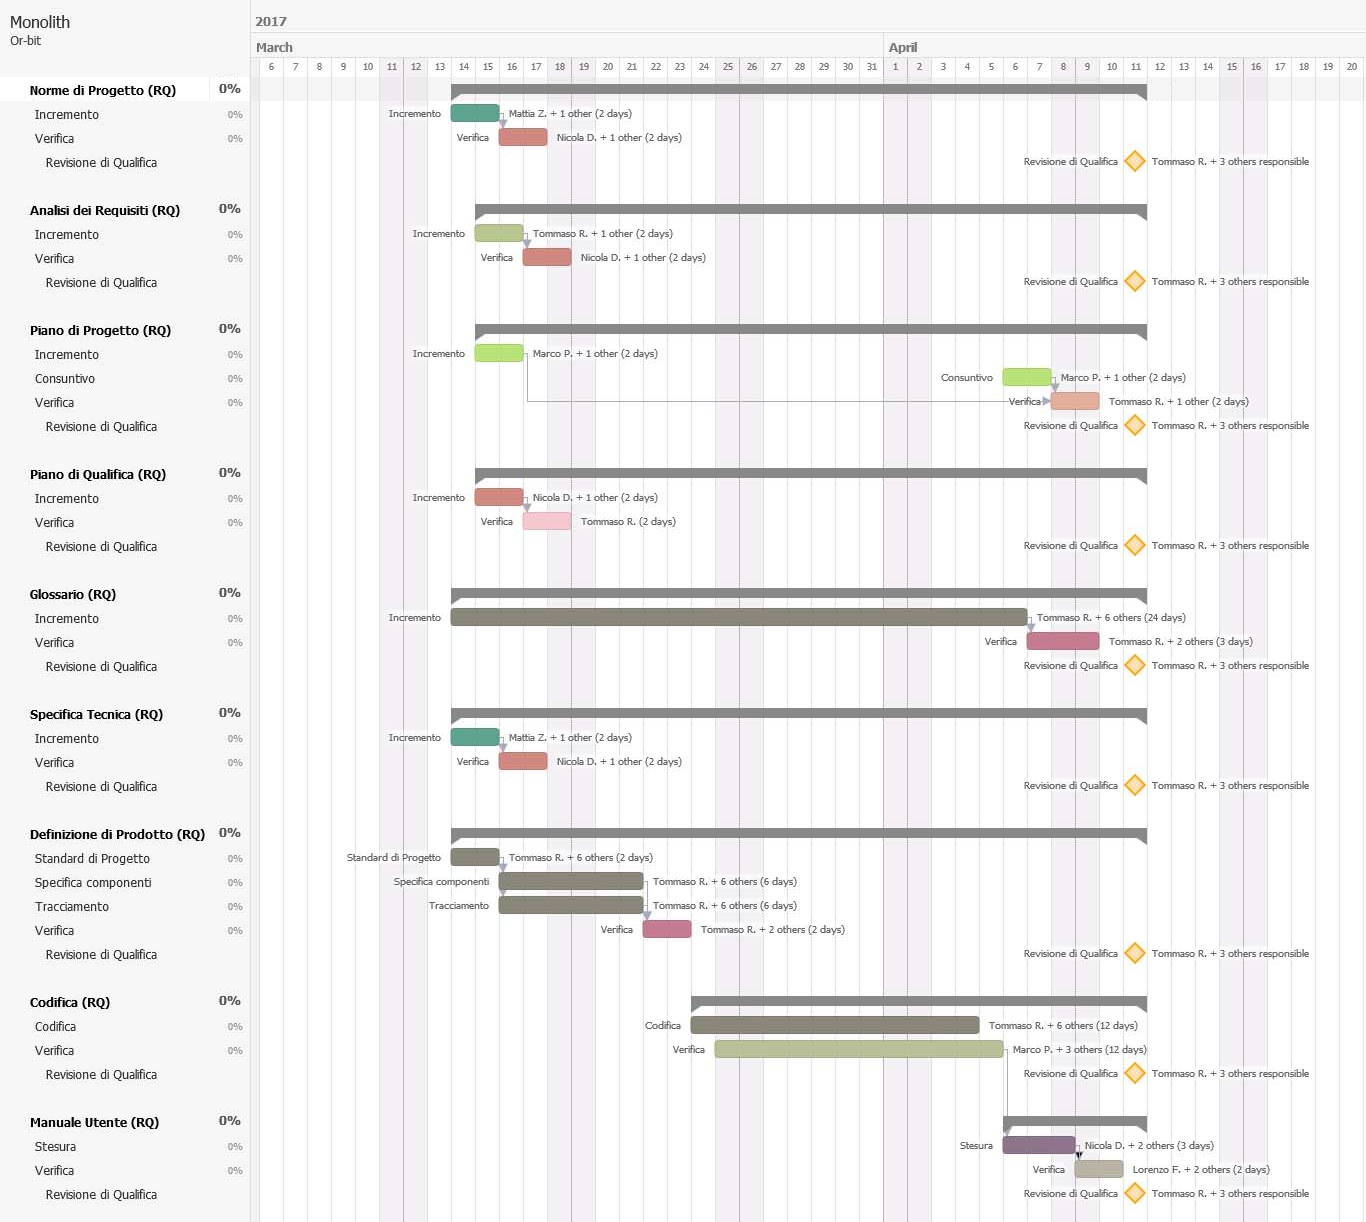
\includegraphics{gantt/Gantt_RQ.png}}
	\caption{Diagramma di Gantt, fase di \PD{} e \Cod{}}
\end{figure}

\subsubsection{Ripartizione ore}
\bgroup
\begin{longtable}{|l|l|l|c|}
	\endfirsthead
	\hline
	\textbf{Identificativo} &
	\textbf{Nome Attività} &
	\textbf{Ruolo} &
	\textbf{Ore}\\
	\endhead
	\hline
	\textbf{RQ1} & \textbf{Norme di Progetto} &  &  \\
	\hline
	{RQ1.1} & {Incremento} & Amministratore  & 3\\
	\hline
	{RQ1.2} & {Verifica} & Verificatore & 1 \\
	\hline
	\textbf{RQ2} & \textbf{Analisi dei requisiti}  & & \\
	\hline
	{RQ2.1} & {Incremento} & Analista &  3\\
	\hline
	{RQ2.2} & {Verifica} & Verificatore & 1 \\
	\hline
	\textbf{RQ3} & \textbf{Piano di progetto} & &  \\
	\hline
	{RQ3.1} & {Incremento} & Responsabile  &  2\\
	\hline
	{RQ3.2} & {Consuntivo} & Responsabile  &  2\\
	\hline
	{RQ3.3} & {Verifica} & Verificatore  &  3\\
	\hline
	\textbf{RQ4} & \textbf{Piano di qualifica} & &  \\
	\hline
	{RQ4.1} & {Incremento} & Progettista  & 8\\
	\hline
	{RQ4.2} & {Verifica} & Verificatore & 2 \\
	\hline
	\textbf{RQ5} & \textbf{Specifica tecnica} & &  \\
	\hline
	{RQ5.1} & {Incremento} & Progettista  & 9\\
	\hline
	{RQ5.2} & {Verifica} & Verificatore & 2 \\
	\hline
	\textbf{RQ6} & \textbf{Definizione di prodotto} & &  \\
	\hline
	{RQ6.1} & {Standard di progetto} & Progettista  & 25\\
	\hline
	{RQ6.2} & {Specifica componenti} & Progettista & 25 \\
	\hline
	{RQ6.3} & {Tracciamento} & Progettista & 25 \\
	\hline
	{RQ6.4} & {Verifica} & Verificatore & 5 \\
	\hline
	\textbf{RQ7} & \textbf{Codifica} & &  \\
	\hline
	{RQ7.1} & {Codifica} & Programmatore  & 120\\
	\hline
	{RQ7.2} & {Verifica} & Verificatore & 5 \\
	\hline
	\textbf{RQ8} & \textbf{Manuale utente} & &  \\
	\hline
	{RQ8.1} & {Stesura} & Amministratore  & 5\\
	& & Programmatore &  10\\
	& & Progettista &  10\\
	\hline
	{RQ8.2} & {Verifica} & Verificatore & 2 \\
	& & Responsabile & 4 \\
	\hline
	\textbf{RQ9} & \textbf{Glossario} & &  \\
	\hline
	{RQ9.1} & {Verifica} & Verificatore &  4 \\
	\hline
	\\
	\caption{Ripartizione ore fase di \PD{} e \Cod{}}
\end{longtable}
\egroup

\subsection{\VV}
\textbf{Periodo:} da 19-04-2017 a 08-05-2017 \\
La fase di \VV{} è la fase finale del progetto, prevede la verifica di tutto il sistema realizzato.
Nella fase di Analisi i ruoli maggiormente coinvolti sono \Programmatore{}, \Progettista{}, \Responsabile{}, \Amministratore{} e \Verificatore{}.
\subsubsection{Gantt attività}
\begin{figure}[H]
	\centering
	\scalebox{0.3}{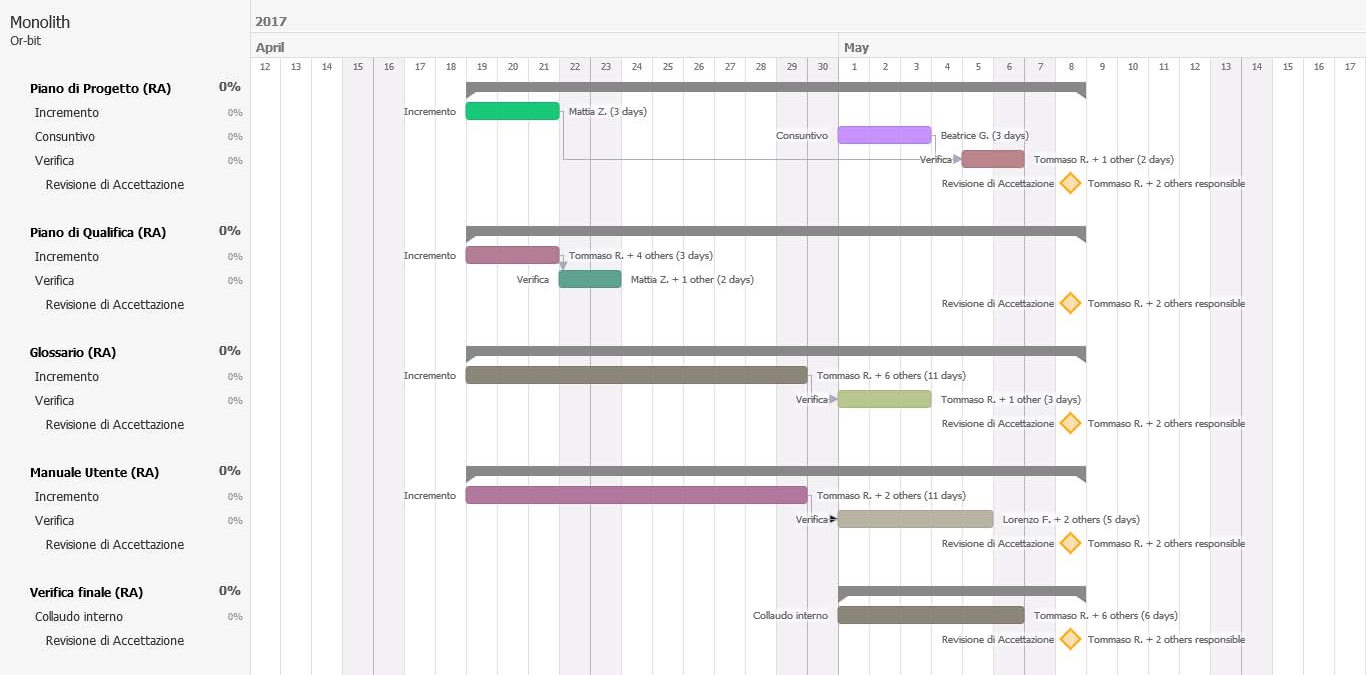
\includegraphics{gantt/Gantt_RA.png}}
	\caption{Diagramma di Gantt, fase di \VV{}}
\end{figure}

\subsubsection{Ripartizione ore}
\bgroup
\begin{longtable}{|l|l|l|c|}
	\endfirsthead
	\hline
	\textbf{Identificativo} &
	\textbf{Nome Attività} &
	\textbf{Ruolo} &
	\textbf{Ore}\\
	\endhead
	\hline
	\textbf{RA1} & \textbf{Piano di progetto} &  &  \\
	\hline
	{RA1.1} & {Incremento} & Responsabile  & 1\\
	\hline
	{RA1.1} & {Consuntivo} & Responsabile  & 1\\
	\hline
	{RA1.2} & {Verifica} & Verificatore & 5 \\
	\hline
	\textbf{RA2} & \textbf{Piano di Qualifica}  & & \\
	\hline
	{RA2.1} & {Incremento} & Responsabile &  1\\
	\hline
	{RA2.2} & {Verifica} & Verificatore & 5 \\
	\hline
	\textbf{RA3} & \textbf{Manuale utente} & &  \\
	\hline
	{RA3.1} & {Incremento} & Amministratore  &  5\\
	& & Progettista & 4 \\
	\hline
	{RA3.2} & {Verifica} & Verificatore  &  5\\
	& & Responsabile & 2 \\
	\hline
	\textbf{RA4} & \textbf{Piano di Qualifica}  & & \\
	\hline
	{RA4.1} & {Collaudo} & Responsabile &  5\\
	& & Amministratore & 5 \\
	& & Programmatore & 10 \\
	& & Verificatore & 40 \\
	\hline
	\textbf{RA5} & \textbf{Glossario} & &  \\
	\hline
	{RA5.1} & {Verifica} & Verificatore &  4 \\
	\hline
	\\
	\caption{Ripartizione ore fase di \VV{}}
\end{longtable}
\egroup
